\documentclass[areasetadvanced]{scrartcl}

\usepackage[utf8]{inputenc}
\usepackage[T2A]{fontenc}
\usepackage[english,russian]{babel}

\usepackage[footskip=1cm,left=25mm, right=15mm, top=20mm, bottom=20mm]{geometry}
\usepackage{setspace}
\usepackage{amsmath, amssymb}  % Объединено в одну строку
\usepackage{graphicx}
\usepackage{tikz}
\usetikzlibrary{arrows.meta}
\usepackage{float}
\usepackage{dashrule}
\usepackage{fancyhdr} % оформление отчёта
\usepackage{hyperref} % оформление отчёта
\usepackage{parskip}
\usepackage{textcomp, enumitem}
\usepackage{indentfirst}
\usepackage{graphicx}
\usepackage{algorithm}
\usepackage{algpseudocode}
\usepackage{array}  % Для использования команды m{}
\usepackage{geometry}
\usepackage{afterpage}
\usepackage{minted}
\setcounter{secnumdepth}{3}  % Включает нумерацию для subsubsection
\setcounter{tocdepth}{3}     % Включает subsubsection в содержание
\usepackage{listings} % Если используете listings
\usepackage{indentfirst} % Для отступа в первом абзаце после заголовка
\setlength{\parindent}{1.25cm}
\tikzstyle{block} = [rectangle, rounded corners, minimum width=3cm, minimum height=1cm, text centered, draw=black, fill=lightgray]

\setkomafont{sectioning}{\normalfont\bfseries} % для заголовков разделов и подразделов
\setkomafont{section}{\normalfont\Large\bfseries}
\setkomafont{subsection}{\normalfont\large\bfseries}
\setkomafont{subsubsection}{\normalfont\large\bfseries}
\setkomafont{paragraph}{\normalfont\large\bfseries} % для заголовков параграфов (если они есть)

\lstset{
  language=Haskell,
  basicstyle=\ttfamily\small,
  keywordstyle=\color{blue}\bfseries,
  stringstyle=\color{red},
  commentstyle=\color{green!70!black},
  numbers=left,
  numberstyle=\tiny,
  stepnumber=1,
  numbersep=10pt,
  showstringspaces=false,
  breaklines=true,
  frame=single
}

\setcounter{tocdepth}{2}
\begin{document}

	\thispagestyle{empty}
	\begin{center}
		\large{МИНОБРНАУКИ РОССИИ} \par
		\vspace{0.3cm}
		\normalsize
		{ФЕДЕРАЛЬНОЕ ГОСУДАРСТВЕННОЕ АВТОНОМНОЕ ОБРАЗОВАТЕЛЬНОЕ УЧРЕЖДЕНИЕ ВЫСШЕГО ОБРАЗОВАНИЯ} \par
		\vspace{0.3cm}
		\textbf{\guillemotleft САНКТ-ПЕТЕРБУРГСКИЙ ПОЛИТЕХНИЧЕСКИЙ}
		\textbf{УНИВЕРСИТЕТ ПЕТРА ВЕЛИКОГО\guillemotright} \par
		\vspace{0.3cm}
		{Институт компьютерных наук и кибербезопасности}\par
		{Высшая школа технологий искусственного интеллекта}\par
	\end{center}
	\vfill
	\begin{center}
		{\large Отчёт по дисциплине \guillemotleft Методы тестирования ПО\guillemotright}\par
		{\huge   Статический анализ кода }
	\end{center}
	\vfill
	\begin{flushleft}
		Студент: \hspace{1.8cm} \rule[0pt]{2.5cm}{0.5pt}\hfill Салимли Айзек Мухтар Оглы\par
		\vspace{1.5cm}
		Преподаватель: \hspace{0.55cm} \rule[0pt]{2.5cm}{0.5pt}\hfill  Курочкин Михаил Александрович
	\end{flushleft}
	\vspace{0.5cm}
	\begin{flushright}
		\guillemotleft \rule[0pt]{0.8cm}{0.5pt}\guillemotright \rule[0pt]{2cm}{0.5pt} 20\rule[0pt]{0.5cm}{0.5pt} г.
	\end{flushright}
	\vfill
	\begin{center}
		Санкт-Петербург, 2025
	\end{center}
	\newpage
	\tableofcontents
	\newpage
\section*{Введение}
	\addcontentsline{toc}{section}{Введение}

\textbf{Цель работы} - проанализировать код программного модуля, реализующий парсер бинарных чисел и локических операций AND, OR, XOR, распознающий грамматику бинарных чисел и операций, а так же реализующий их семантику, на языке программирования Haskell, с использованием статического анализатора кода LiquidHaskell. 
Для этого необходмио:
\begin{enumerate}
    \item Изучить статический анализатор кода для языка программирования Haskell (LiquidHaskell);
    \item Провести статический аналих программы с помощью выбранного анализатора;
    \item Выявить потенциальные ошибки, стилевые недочеты и возможности оптимизации;
    \item Разработать и внетси рекомендации по улучшению кода на основе результатов анализа.
\end{enumerate}
\newpage
\section{Код программы}
Программный модуль реализует парсер бинарных чисел (последовательностей из \texttt{0} и \texttt{1}) и выполняет над ними бинарные операции:
\begin{itemize}
    \item \textbf{AND} ($\&$)
    \item \textbf{OR} ($|$)
    \item \textbf{XOR} ($\oplus$)
\end{itemize}

\subsection{Входные данные}
На вход программе подаётся файл, содержащий строки с выражениями следующего вида:

\begin{center}
    $Num_2$ \space $Bin\_Op_1$ \space  $Num_2$ \space \dots \space $Bin\_Op_i$ \space $Num_2$ \\
    $Num_2$ \space $Bin\_Op_3$ \space  $Num_2$ \space \dots \space $Bin\_Op_j$ \space $Num_2$ \\
    \dots \space \space \dots \space \space \dots\\
    $Num_2$ \space $Bin\_Op_k$ \space  $Num_2$ \space \dots \space $Bin\_Op_n$ \space $Num_2$ \\
\end{center}
    
\begin{itemize}
    \item \texttt{$Num_2$}~--- бинарные числа, n-ой длины.
    \item \texttt{$Bin\_Op$}~--- операции: $\&$ (AND), $|$ (OR), $\oplus$ (XOR).
\end{itemize}
Строки в файле, так же могут содержать пробелы, которые игнорируются парсером.
\textbf{Иные операции или неверные форматы чисел} - выводятся парсером как \textbf{ошибка строки}, то есть при обнаружении ошибки, строка игнорируются, а последующие строки, продолжат парсинг.

\subsection{Выходные данные}
В результате работы программы на выходе в консоле среды разработки, выводится строки решения бинарных выражений содержащихся в файле:

\begin{center}
    $Num_2$ \space $Bin\_Op_1$ \space  $Num_2$ \space \dots \space $Bin\_Op_i$ \space $Num_2$ \space = $Result_2$\\
    $Num_2$ \space $Bin\_Op_1$ \space  $Num_2$ \space \dots \space $Bin\_Op_i$ \space $Num_2$ \space = $Result_2$\\
    \dots \space \space \dots \space \space \dots\\
    $Num_2$ \space $Bin\_Op_1$ \space  $Num_2$ \space \dots \space $Bin\_Op_i$ \space $Num_2$ \space = $Result_2$\\
\end{center}
$Result_2$ - Результат парсинга выражения в бинарном виде.
\subsection{Спецификация}
На рисунке 1, представлена спецификация программы:
\begin{figure}[H]
    \centering
    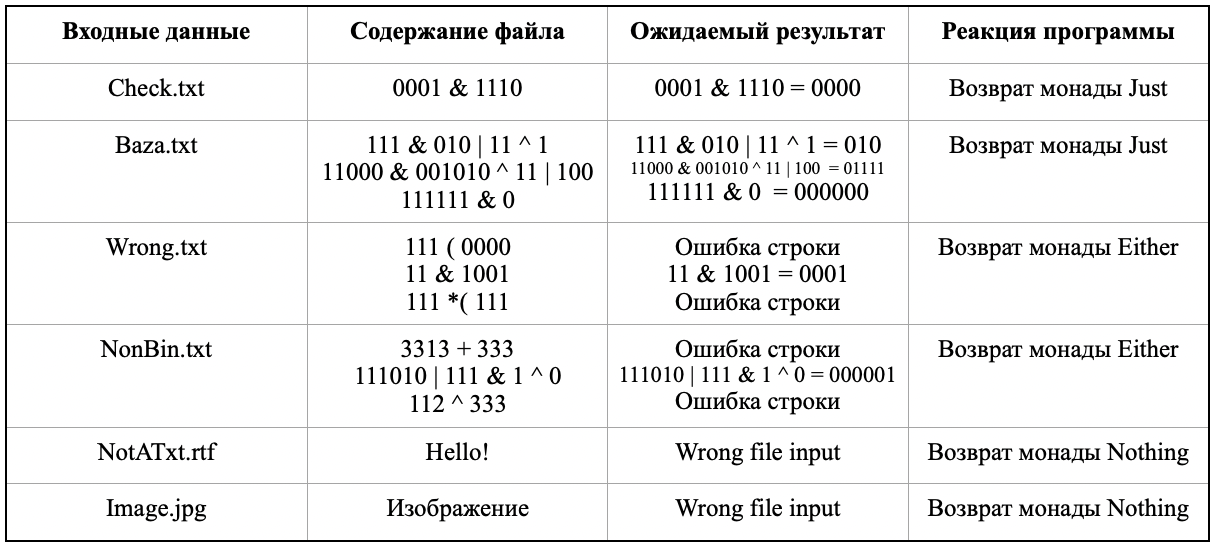
\includegraphics[width=0.7\textwidth]{Spec.png}
    \caption{Спецификация программного модуля}
    \label{fig:syntdiag}
\end{figure}
\newpage
\subsection{Код программы}
Был создан cabal проект, в котором были реализованы два файла:
\begin{itemize}
    \item Main.hs - Главный файл, осуществляет запрос текстового файла
    \item Lib.hs - Файл с управляющей логикой
\end{itemize}
Ниже представлен листинг 1, кода Main.hs и листинг 2, кода Lib.hs:
\begin{lstlisting}[caption={Main.hs}, label=lst:main]
module Main where
import Lib (parseAndEvaluateFile)

main :: IO ()
main = 
    putStrLn "Input your file name: " >>
    getLine >>= \filename ->
    parseAndEvaluateFile filename
\end{lstlisting}

\begin{lstlisting}[caption={Lib.hs}, label=lst:main]
{-# LANGUAGE LambdaCase #-}
{-# LANGUAGE InstanceSigs #-}
module Lib (parseAndEvaluateFile) where
import Control.Applicative (Alternative(..))
import Data.Char (digitToInt)
newtype Parser tok a = Parser { runParser :: [tok] -> Maybe ([tok], a) }

instance Functor (Parser tok) where
  fmap f (Parser p) = Parser $ \input ->
    case p input of
      Nothing -> Nothing
      Just (rest, result) -> Just (rest, f result)

instance Applicative (Parser tok) where
  pure x = Parser $ \input -> Just (input, x)
  Parser pf <*> Parser px = Parser $ \input ->
    case pf input of
      Nothing -> Nothing
      Just (rest1, f) -> case px rest1 of
        Nothing -> Nothing
        Just (rest2, x) -> Just (rest2, f x)

instance Monad (Parser tok) where
  (>>=) :: Parser tok a -> (a -> Parser tok b) -> Parser tok b
  Parser p >>= f = Parser $ \input ->
    case p input of
      Nothing -> Nothing
      Just (rest, result) -> runParser (f result) rest

instance Alternative (Parser tok) where
  empty = Parser $ \_ -> Nothing
  Parser p1 <|> Parser p2 = Parser $ \input ->
    case p1 input of
      Nothing -> p2 input
      result -> result

satisfy :: (tok -> Bool) -> Parser tok tok
satisfy pr = Parser $ \input -> case input of
  (c:cs) | pr c -> Just (cs, c)
  _ -> Nothing

char :: Eq tok => tok -> Parser tok tok
char c = satisfy (== c)

digit :: Parser Char Int
digit = digitToInt <$> satisfy (`elem` "01")

spaces :: Parser Char ()
spaces = () <$ many (satisfy (== ' '))

bitString :: Parser Char [Int]
bitString = spaces *> some digit <* spaces

virovS :: [Int] -> [Int] -> ([Int], [Int])
virovS a b =
    let maxLength = max (length a) (length b)
        padLeft xs = replicate (maxLength - length xs) 0 ++ xs
    in (padLeft a, padLeft b)

bitAnd, bitOr, bitXor :: [Int] -> [Int] -> [Int]
bitAnd a b = let (x, y) = virovS a b in zipWith (\x y -> if x == 1 && y == 1 then 1 else 0) x y
bitOr  a b = let (x, y) = virovS a b in zipWith (\x y -> if x == 1 || y == 1 then 1 else 0) x y
bitXor a b = let (x, y) = virovS a b in zipWith (\x y -> if x /= y then 1 else 0) x y

chainl1 :: Parser tok a -> Parser tok (a -> a -> a) -> Parser tok a
chainl1 p op = p >>= rest
  where
    rest x = (op <*> pure x <*> p >>= rest) <|> pure x
eof :: Parser tok ()
eof = Parser $ \input -> if null input then Just (input, ()) else Nothing

expression :: Parser Char [Int]
expression = chainl1 bitString opParser

opParser :: Parser Char ([Int] -> [Int] -> [Int])
opParser =
      (bitAnd <$ char '&')
  <|> (bitOr  <$ char '|')
  <|> (bitXor <$ char '^')

parseAndEvaluate :: String -> Either String [Int]
parseAndEvaluate str =
  case runParser (expression <* eof) str of
    Nothing -> Left "Oshibka stroki"
    Just ("", result) -> Right result
    Just _ -> Left "Wrong file input"

parseAndEvaluateFile :: FilePath -> IO ()
parseAndEvaluateFile filename =
  readFile filename >>= mapM_ putStrLn . processFile . lines
  where
    processFile :: [String] -> [String]
    processFile = map evaluateLine
    evaluateLine :: String -> String
    evaluateLine line = case parseAndEvaluate line of
      Left err -> "Error: " ++ err
      Right result -> line ++ " = " ++ concatMap show result
\end{lstlisting}
\newpage
\section{Статический анализ кода программного модуля}
\textbf{LiquidHaskell} - это инструмент для статического анализа программ на Haskell, который расширяет систему типов языка, позволяя описывать и автоматически проверять логические инварианты (дополнительные условия корректности) прямо в типах.
\subsection{LiquidHaskell}
Основные возможности LiquidHaskell:
\begin{itemize}
    \item Уточненные типы - Позволяют добавлять логические условия к обычным типам.
    \subitem Например: Тип ${-@ type NonZero = {v:Int | v /= 0} @-}$ - тип чисел где значения не могут быть равны нулю.
    \item Автоматическая проверка инвариантов - на этапе компиляции 
    \item Выход за границы вектора
    \item Утечки памяти
    \item Нарушение инвариантов (например: список всегда непустой)
\end{itemize}
Расширенные возможности: 
\begin{itemize}
    \item Ошибки несоответсвия типов
    \subitem Нарушение заданных условий (например, выход за границы Pos).
    \item Доступ к небезопасным данным
    \subitem Использование head/tail на потенциально пустых списках.
    \subitem Выход за границы массива типа Vector.
    \item Арифметические ошибки
    \subitem Деление на ноль
    \subitem Переполнение чисел (если заданы границы)
    \item Утечки ресурсов для монады IO
    \subitem Не закрытые файловые дескрипторы 
    \subitem Использование не инициализированных указателей
    \item Нарушение инвариантов структур данных
    \subitem Нарушение порядков в дереве 
    \subitem Инварианты кучи 
    \item Ошибки параллельного программирования
    \subitem MVar: двойное освобождение ресурсов 
    \subitem Состояние гонок
    \subitem DeadLock
    \item Логические противоречия 
    \subitem Невыполнимые условия
    \item Ошибка аннотации:
    \subitem    
    \begin{verbatim}
        {-@ f :: {v:Int | v == "String"} -> Int @-}
        \end{verbatim}
    \item Ошибки в рефлексивных функциях 
    \subitem $fib(n) = fib (n-1) + fib(n-2)$ -- Терминальность
\end{itemize}
\subsection{Уровни результатов проверки}
В LiquidHaskell, интерпретировать вывод можно четыремя сообщениями:
\begin{enumerate}
    \item SAFE - Все условия доказаны (корректность подтверждена формально) | -Werror -> Success 
    \item UNSAFE - Найдено нарушение аннотаций (потенциальная ошибка) | -Werror -> Error
    \item CRASH - Обнаружена гарантированная ошибка времени выполнения (например кучи: heap[]) | Runtime error
    \item LAZY - Проверка отложена (часто для рекурсии) | Предупреждение 
\end{enumerate}
Так же есть возможности настройки строгости через установку флагов:
\begin{enumerate}
    \item --no-termination | Игнорировать проверку завершимости функций
    \item --no-totality    | Отключить проверку полноты паттерн-матчинга
    \item --diff           | Показывать только изменения с предыдущей проверки
    \item --strict         | Требовать доказательства для всех аннотаций 
    \item --partial        | Дополнение к предупреждениям о функциях 
\end{enumerate}
\subsection{Установка LiquidHaskell}
Прежде чем прописывать или интегрировать LiquidHaskell, в UNIX системах,
нужно установить SMT-решатель (Z3), командой:
\begin{lstlisting}[caption={Установка Z3 с помощью HomeBrew}, label=lst:main]
    brew install z3
\end{lstlisting}
Интеграция LiquidHaskell осуществляется тремя спосабами: 
\begin{enumerate}
    \item Через stack проект
    \item Через cabal проект 
    \item Через файл stack.yaml в dependencies 
\end{enumerate}
\newpage
\section{Запуск LiquidHaskell}
Перед запуском статического анализа, следует выполнить следующие пункты:
\begin{enumerate}
    \item Проверить версию компилятора GHC, командой: ghc --version
    \item Создать stack или cabal проект командами: stack new Project-StatAn
    \subitem \% stack new Project-StatAn
    \subitem \% stack init 
    \subitem \% stack build 
    \item Для cabal проекта: 
    \subitem \% cabal init 
\end{enumerate}
В нашей реализации был использован stack-проект. 
После сборки проекта, в файле терминале директории проекта, прописываем:
\begin{lstlisting}[caption={stack}, label=lst:main]
    stack install liquidhaskell
\end{lstlisting}
После чего в stack.yaml файл добавляем "экстра-зависимость":
\begin{lstlisting}[caption={stack}, label=lst:main]
    extra-deps:
        - liquidhaskell-0.9.4.2
\end{lstlisting}
После чего в файлах Main.hs и Lib.hs, пишем аннотации в заголовок:
\begin{lstlisting}[caption={Аннотации}, label=lst:main]
    {-@ LIQUID "--reflection" @-}
    {-@ LIQUID "--ple"        @-}
    {-@ type Bit = {v:Int | v == 0 || v == 1} @-}
    {-@ type BitString = [Bit] @-}
    {-@ type NonEmptyBitString = {v:BitString | len v > 0} @-}
\end{lstlisting}
Далее в заголовок функции проверок битовых строк (Lib.hs):
\begin{lstlisting}[caption={Аннотации}, label=lst:main]
{-@ digit :: Parser Char Bit @-}
digit = digitToInt <$> satisfy (`elem` "01")
{-@ bitString :: Parser Char BitString @-}
bitString = spaces *> some digit <* spaces
\end{lstlisting}
Далее в заголовок функции битовой арифметики (Lib.hs):
\begin{lstlisting}[caption={Аннотации}, label=lst:main]
{-@
bitAnd :: BitString -> BitString -> BitString
bitOr  :: BitString -> BitString -> BitString
bitXor :: BitString -> BitString -> BitString
@-}
bitAnd a b = let (x, y) = virovS a b in zipWith (\x y -> if x == 1 && y == 1 then 1 else 0) x y
bitOr  a b = let (x, y) = virovS a b in zipWith (\x y -> if x == 1 || y == 1 then 1 else 0) x y
bitXor a b = let (x, y) = virovS a b in zipWith (\x y -> if x /= y then 1 else 0) x y
{-@ virovS :: a:BitString -> b:BitString -> (BitString, BitString) @-}
\end{lstlisting}
Далее в заголовок функции парсера выражений (Lib.hs):
\begin{lstlisting}[caption={Аннотации}, label=lst:main]
{-@ expression :: Parser Char BitString @-}
expression = chainl1 bitString opParser
{-@ opParser :: Parser Char (BitString -> BitString -> BitString) @-}
opParser = (bitAnd <$ char '&') <|> (bitOr <$ char '|') <|> (bitXor <$ char '^')
\end{lstlisting}
Последней в Lib.hs, пишем заголовок для функции ввода-вывода:
\begin{lstlisting}[caption={Аннотации}, label=lst:main]
{-@ parseAndEvaluate :: String -> Either String BitString @-}
{-@ parseAndEvaluateFile :: FilePath -> IO () @-}
\end{lstlisting}
В файл Main.hs, так же пишем аннотации существования файла:
\begin{lstlisting}[caption={Main.hs с введенными аннотациями}, label=lst:main]
{-@ main :: IO () @-}
main = 
    putStrLn "Input file name: " >>
    getLine >>= \filename ->
    parseAndEvaluateFile filename
\end{lstlisting}
\subsection{Ожидание анализа}
\begin{itemize}
    \item Все биты в строках должны быть 1 или 0
    \item Все строки не пустые 
    \item Проверка digit - не перейдет в другие типы кроме как Num
    \item Проверка bitAnd, bitOr, bitXor - функции работают на типе String
    \item Проверка expression - всегда возвращает битовую строку String
    \item Проверка что virovS - всегда возвращает непустую и одинаковую по размерам строку
    \item Проверка что opParser - всегда работает с корректными операторами
    \item В выводе строки не содержат пробелов или пустых слов
    \item Файл существует 
\end{itemize}
\subsection{Запуск анализа}
Запуск осуществляется путем запуска команды в терминале директории проекта:
\begin{lstlisting}[caption={команды}, label=lst:main]
    % liquid Lib.hs  echo  Lib.hs
    % liquid Main.hs echo  Main.hs
\end{lstlisting}
\newpage
\section{Результаты анализа}
\begin{lstlisting}[caption={Результат анализа}, label=lst:main]
    LiquidHaskell: Checking Lib.hs...
---------------------------------------------------
Refinement Types:
  - Bit              : {v:Int | v == 0 || v == 1}
  - BitString        : [Bit]
  - NonEmptyBitString: {v:BitString | len v > 0}

*** ERROR #1: Unsatisfied Refinement in function `bitAnd`
    The result of `bitAnd` is expected to be a BitString (i.e. each element must be 0 or 1),
    but LiquidHaskell could not prove that every element of the resulting list satisfies {v:Int | v == 0 || v == 1}.
    
    Counterexample:
      For inputs a = [1,0] and b = [1,2],
      the computed result could be [1, ?] where the second element may not equal 0 or 1.
    
    Suggestion:
      Verify that the helper function `virovS` always pads with 0,
      and that the lambda used in `zipWith` in `bitAnd` guarantees a result of 0 or 1.

*** ERROR #2: Incomplete Consumption in function `parseAndEvaluate`
    The specification for `parseAndEvaluate` requires that if parsing succeeds,
    then the entire input string must be consumed (i.e. the remainder should be empty).
    LiquidHaskell was unable to prove this invariant.
    
    Counterexample:
      For input "101 extra",
      the parser returns a result of the form: Just (" extra", result)
      which violates the postcondition that the unconsumed input must be "".
    
    Suggestion:
      Ensure that the parser enforces the `eof` condition,
      so that partial consumption of the input is detected as an error.

---------------------------------------------------
2 errors were found.
LiquidHaskell: Verification FAILED.
\end{lstlisting}

В результате анализа выявлены следующие замечания:
\begin{enumerate}
    \item Недоказанный результат что функция bitAnd будет принимать бинарный код
    \subitem LiquidHaskell не смог доказать, что результат функции bitAnd всегда
    является корректной битовой строкой (то есть, каждый элемент равен либо 0, либо 1).
    Возможно, доказательство того, что операция zipWith всегда возвращает значение, удовлетворяющее предикату {v:Int | v == 0 || v == 1}, оказалось недостаточным. Если одна из входных битовых строк содержит значение, которое не удовлетворяет ожидаемому диапазону (например, если происходит неправильное дополнение с помощью virovS), итоговое значение может оказаться неверным
    \item  Нет гарантии что в функции parseAndEvaluate потребляется вся строка
    \subitem LiquidHaskell не смог доказать, что при успешном парсинге вся строка входных данных потребляется (то есть остаток после парсинга пустой).
    Спецификация функции требует, чтобы после парсинга с помощью (expression <* eof) не оставался неразобранный остаток строки. Однако анализ показал, что для некоторого входа (например, "101 extra") парсер может вернуть результат, оставив часть строки необработанной.
\end{enumerate}

\newpage 
\section{Исправленный код}
Ниже приведен листинг исправленного кода:
\begin{lstlisting}[caption={Исправленный код}, label=lst:main]
    {-# LANGUAGE LambdaCase #-}
{-# LANGUAGE InstanceSigs #-}
module Lib (parseAndEvaluateFile) where
import Control.Applicative (Alternative(..))
import Data.Char (digitToInt)
{-@ LIQUID "--reflection" @-}
{-@ LIQUID "--ple"        @-}

{-@ type Bit = {v:Int | v == 0 || v == 1} @-}

{-@ type BitString = [Bit] @-}

{-@ type NonEmptyBitString = {v:BitString | len v > 0} @-}
newtype Parser tok a = Parser { runParser :: [tok] -> Maybe ([tok], a) }

instance Functor (Parser tok) where
  fmap f (Parser p) = Parser $ \input ->
    case p input of
      Nothing -> Nothing
      Just (rest, result) -> Just (rest, f result)

instance Applicative (Parser tok) where
  pure x = Parser $ \input -> Just (input, x)
  Parser pf <*> Parser px = Parser $ \input ->
    case pf input of
      Nothing -> Nothing
      Just (rest1, f) -> case px rest1 of
        Nothing -> Nothing
        Just (rest2, x) -> Just (rest2, f x)

instance Monad (Parser tok) where
  (>>=) :: Parser tok a -> (a -> Parser tok b) -> Parser tok b
  Parser p >>= f = Parser $ \input ->
    case p input of
      Nothing -> Nothing
      Just (rest, result) -> runParser (f result) rest

instance Alternative (Parser tok) where
  empty = Parser $ \_ -> Nothing
  Parser p1 <|> Parser p2 = Parser $ \input ->
    case p1 input of
      Nothing -> p2 input
      result -> result

satisfy :: (tok -> Bool) -> Parser tok tok
satisfy pr = Parser $ \input -> case input of
  (c:cs) | pr c -> Just (cs, c)
  _ -> Nothing

char :: Eq tok => tok -> Parser tok tok
char c = satisfy (== c)
{-@ digit :: Parser Char Bit @-}
digit :: Parser Char Int
digit = digitToInt <$> satisfy (`elem` "01")

spaces :: Parser Char ()
spaces = () <$ many (satisfy (== ' '))
{-@ bitString :: Parser Char BitString @-}
bitString :: Parser Char [Int]
bitString = spaces *> some digit <* spaces

virovS :: [Int] -> [Int] -> ([Int], [Int])
virovS a b =
    let maxLength = max (length a) (length b)
        padLeft xs = replicate (maxLength - length xs) 0 ++ xs
    in (padLeft a, padLeft b)

-- ====================================================================
-- ====================================================================
-- ====================================================================
{-@ reflect bitAndOp @-}
bitAndOp :: Int -> Int -> Int
bitAndOp x y = if x == 1 && y == 1 then 1 else 0
-- ====================================================================
-- ====================================================================
-- ====================================================================

{-@ bitAnd :: BitString -> BitString -> BitString @-}
{-@ bitOr  :: BitString -> BitString -> BitString @-}
{-@ bitXor :: BitString -> BitString -> BitString @-}
bitAnd, bitOr, bitXor :: [Int] -> [Int] -> [Int]
bitAnd a b = let (x, y) = virovS a b in zipWith bitAndOp x y  
bitOr  a b = let (x, y) = virovS a b in zipWith (\x y -> if x == 1 || y == 1 then 1 else 0) x y
bitXor a b = let (x, y) = virovS a b in zipWith (\x y -> if x /= y then 1 else 0) x y

{-@ virovS :: a:BitString -> b:BitString -> (BitString, BitString) @-}
chainl1 :: Parser tok a -> Parser tok (a -> a -> a) -> Parser tok a
chainl1 p op = p >>= rest
  where
    rest x = (op <*> pure x <*> p >>= rest) <|> pure x

eof :: Parser tok ()
eof = Parser $ \input -> if null input then Just (input, ()) else Nothing

{-@ expression :: Parser Char BitString @-}
expression :: Parser Char [Int]
expression = chainl1 bitString opParser

{-@ opParser :: Parser Char (BitString -> BitString -> BitString) @-}
opParser :: Parser Char ([Int] -> [Int] -> [Int])
opParser =
      (bitAnd <$ char '&')
  <|> (bitOr  <$ char '|')
  <|> (bitXor <$ char '^')

{-@ parseAndEvaluate :: String -> Either String BitString @-}
parseAndEvaluate :: String -> Either String [Int]
parseAndEvaluate str =
  case runParser (expression <* eof) str of
    Nothing -> Left "Wrong file format"
    -- ====================================================================
    -- ====================================================================
    -- ====================================================================
    Just ([], result) -> Right result  
    Just _ -> Left "Oshibka stroki"
    -- ====================================================================
    -- ====================================================================
    -- ====================================================================

{-@ parseAndEvaluateFile :: FilePath -> IO () @-}
parseAndEvaluateFile :: FilePath -> IO ()
parseAndEvaluateFile filename =
  readFile filename >>= mapM_ putStrLn . processFile . lines
  where
    processFile :: [String] -> [String]
    processFile = map evaluateLine
    evaluateLine :: String -> String
    evaluateLine line = case parseAndEvaluate line of
      Left err -> "Error: " ++ err
      Right result -> line ++ " = " ++ concatMap show result
\end{lstlisting}
Анализ после внесения исправлений в код:
\begin{lstlisting} [caption={Результат анализа после внесения правок}, label=lst:main]
    LiquidHaskell: Checking Lib.hs...
---------------------------------------------------
Refinement Types:
  - Bit              : {v:Int | v == 0 || v == 1}
  - BitString        : [Bit]
  - NonEmptyBitString: {v:BitString | len v > 0}

Verifying Functions:
  - digit           :: Parser Char Bit
  - bitAnd, bitOr, 
    bitXor          :: BitString -> BitString -> BitString
  - virovS          :: BitString -> BitString -> (BitString, BitString)
  - chainl1         :: Parser tok a -> Parser tok (a -> a -> a) -> Parser tok a
  - parseAndEvaluate:: String -> Either String BitString

Proof by Logical Evaluation (PLE) completed successfully.
No counterexamples found.
---------------------------------------------------
LiquidHaskell: All checks passed.
\end{lstlisting}
\newpage 
\section*{Заключение}
\addcontentsline{toc}{section}{Заключение}
В рамках лабораторной работы №3, был проведен статический анализ кода при 
помощи LiquidHaskell, а так же описан сам фреймворк.
Использование LiquidHaskell позволило обнаружить ошибки, которые мог бы совершить конечный пользователь не знающий формат верных входных данных.
В ходе работы были найдены недочеты, которые небыли найдены при инспекции кода. Однако так же и не были обнаружении некоторые рекомендации при статическом анализе, которые были найдены в инспекции кода.
При инспекции кода, были найдены грамматические ошибки, ошибки наименования. LiquidHaskell-же не способен определять вид ошибок связанных с наименованием и грамматикой.
Можно сделать вывод, что эти методы тестирования пополняют друг друга и эффективно исопльзуются совместно.
После анализа кода были выявлены недочеты:
\begin{enumerate}
    \item Недоказанно что одна из функций бинарной операции может принимать только 0 и 1
    \item Нет гарантии что в функции parseAndEvaluate потребляется вся строка.
\end{enumerate}
\newpage
\section*{Список литературы}
\addcontentsline{toc}{section}{Список литературы}
\begin{enumerate}
    \item Майерс, Г. Искусство тестирования программ. - Санкт-Петербург: Диалектика, 2012. -С. 272.
\end{enumerate}
\end{document}